\scanpage{88}
U N I V E R S I T E\\
DES SCIENCES ET TECHNIQUES\\
DU LANGUEDOC

\figure{\begin{tikzpicture}\draw[dashed] (0,0)--(2,0);\end{tikzpicture}}

AMC/GJ\\
\uline{Diffusion} : Liste A\\
N°4549

Montpellier, le 16 Juillet 1975

\uline{AVIS DE SOUTENANCE D'UNE THESE DE DOCTEUR-INGENIEUR}

\uline{Nom et prénom du candidat} : DASSOUKI Mouhiddine

\uline{Titre de la thèse} : Etude expérimentale et théorique d'une machine à courant continu à commutation par thyristors tournant avec l'induit.

\uline{Date, heure et lieu de soutenance prévus} :\\
29 Juillet 1975 à 10 Heures\\
Salle de cours n° 9.

\uline{Nom du Directeur de thèse} : R. JOUTY

\uline{Désignation du laboratoire où la thèse est préparée} : Laboratoire de Physique des Métaux.

\uline{Analyse de l'ouvrage} : Il est possible de remplacer le collecteur d'une machine à courant continu classique par une batterie de thyristors. Pour la commande de ces derniers, leurs gachettes sont reliées à un collecteur auxiliaire. L'étude de ce type nouveau de machine fait apparaître des similitudes, mais aussi de grandes différences avec la machine classique; notamment en ce qui concerne la commutation et la réaction d'induit, dont l'auteur donne une analyse très détaillée. L'étude expérimentale, faite sur un prototype obtenu par transformation d'une machine classique, est en bon accord avec la théorie, et fait apparaître des performances satisfaisantes.

\uline{Durée approximative des recherches ayant abouti à la thèse} : 2 ans.

\uline{Composition du jury proposé} :

Monsieur JOUTY R.\\
Monsieur GROUBERT E.\\
Monsieur TROMPETTE

LE SECRETAIRE GENERAL,

\figure{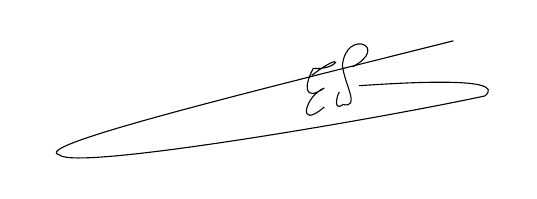
\begin{tikzpicture}[x=1cm,y=1cm]
\draw (5,1.45) .. controls (2,.7) and (-.4,.1) .. (0,0)
.. controls (.2,-.2) and (4,.45) .. (5.4,.75)
.. controls (5.7,1) and (4.4,.92) .. (3.8,.88);
\draw (3.2,1.01) .. controls (3.65,1.36) and (3.55,1.07) .. (3.22,1.1)
.. controls (3.1,.88) and (3.1,.67) .. (3.36,.85)
.. controls (3.12,.76) and (3.0,.3) .. (3.36,.61);
\draw (3.72,1.12) .. controls (4.2,1.38) and (3.64,1.61) .. (3.59,1.14)
.. controls (3.62,.88) and (3.82,.6) .. (3.6,.64)
.. controls (3.47,.55) and (3.52,.75) .. (3.55,.8);
\end{tikzpicture}}

\uline{E. SIAU}

\margin{87}
